% Main document. Compile with XeLaTeX.
\documentclass[10pt,t,aspectratio=169]{beamer}
\usepackage{fontspec}
\setsansfont{lmsans10}[
  Extension=.otf,UprightFont=*-regular,BoldFont=*-bold,
  ItalicFont=*-oblique,BoldItalicFont=*-boldoblique]
\usefonttheme{professionalfonts}
\usepackage{etoolbox}
\usepackage{fvextra}
\setmonofont{Latin Modern Mono}
\usepackage{booktabs,array,tabularx}
\def\slideContentLeftMargin{0.65cm}
\def\slideContentRightMargin{0.65cm}
\def\hustHeaderHeight{1.12cm}
\def\slideContentTopPadding{0cm}
\usepackage[red,169]{beamerthemeHUST}
\usetikzlibrary{arrows.meta,positioning,calc}
% Editable presentation metadata.
\newcommand{\ProjectName}{Hanoi Rent Insight}
\newcommand{\ProjectSubtitle}{Estimating monthly asking rents\\[-0.12em]for apartments and rental rooms}
\newcommand{\PresentationStage}{Capstone Progress Report}
\newcommand{\TeamName}{Capstone Project Team}
\newcommand{\TeamMembers}{%
  Đoàn Trọng Hoà -- 20235935 \\[0.05em]
  Hoàng Danh Thái -- 20235997 \\[0.05em]
  Nguyễn Hữu Tuấn Tú -- 20236005 \\[0.05em]
  Hồ Việt Quang -- 20235991 \\[0.05em]
  Phạm Hiền Mai -- 20235970
}
\newcommand{\LecturerTitle}{Assoc. Prof. Dr.}
\newcommand{\LecturerName}{Than Quang Khoat}
\newcommand{\Advisor}{Lecturer: \LecturerTitle{} \LecturerName}
\newcommand{\ReportDate}{2 November 2026}

\definecolor{ink}{HTML}{252B33}
\definecolor{muted}{HTML}{59616B}
\definecolor{paper}{HTML}{F5F6F7}
\definecolor{line}{HTML}{D7DCE0}
\setbeamercolor{normal text}{fg=ink,bg=white}
\setbeamercolor{structure}{fg=hustprimary}
\setbeamerfont{frametitle}{size=\large,series=\mdseries}
\setbeamertemplate{itemize item}{\small\textbullet}
\setbeamertemplate{navigation symbols}{}
\setbeamertemplate{footline}{\vspace*{0.75cm}}
\newcolumntype{L}[1]{>{\raggedright\arraybackslash}p{#1}}
\newcolumntype{Y}{>{\raggedright\arraybackslash}X}
\setlength{\parskip}{0.20em}
\newenvironment{topicblock}[1]{\par\vspace{0.12cm}{\normalsize\bfseries\color{hustprimary}#1}\par\vspace{0.05cm}}{\par}
\newenvironment{points}{\begin{itemize}\setlength{\itemsep}{0.65em}\setlength{\parsep}{0pt}}{\end{itemize}}
\newcommand{\keyline}[1]{\par\vspace{0.12cm}{\color{hustprimary!30}\rule{\textwidth}{0.4pt}}\par{\small #1}\par}
\newcommand{\smallnote}[1]{{\footnotesize\color{muted}#1}}
\tikzset{flow/.style={->,>=Stealth,line width=0.85pt,draw=hustprimary},
  pipelinebox/.style={draw=hustprimary!50,fill=hustprimary!3,rounded corners=3pt,
    text width=3.65cm,minimum height=1.10cm,align=left,inner sep=7pt,font=\small}}
\patchcmd{\husttitlepage}{Người thực hiện:}{Project team:}{}{\PackageError{HanoiRent}{Title label patch failed}{Check template.}}
\renewcommand{\titlePageTitleX}{-0.3cm}
\renewcommand{\titlePageTitleY}{-0.25cm}
\renewcommand{\hustTitleAlign}{\alignLeft}
\renewcommand{\hustSubtitleAlign}{\alignLeft}
\renewcommand{\hustAuthorAlign}{\alignLeft}
\renewcommand{\hustInstAlign}{\alignLeft}
\title{\ProjectName}
\subtitle{\texorpdfstring{{\normalsize\ProjectSubtitle}\\[-0.15em]{\normalsize\PresentationStage}}{Monthly asking rent estimation -- Capstone Progress Report}}
\author[\TeamName]{\texorpdfstring{\small\TeamMembers}{\TeamName}}
\institute{\vspace{0.3cm}\color{black}\small\normalfont\textbf{Lecturer:} \LecturerTitle{} \LecturerName}
\hypersetup{pdftitle={Hanoi Rent Insight -- Capstone Progress Report},pdfauthor={Đoàn Trọng Hoà; Hoàng Danh Thái; Nguyễn Hữu Tuấn Tú; Hồ Việt Quang; Phạm Hiền Mai},pdfsubject={Objectives, learning problem, proposed pipeline, sample data and actual web interface}}

\begin{document}
% 1: 00:00--00:15
\husttitlepage
\hidePageNumber
\useThinBar
\useStyleLogoOnly

% 2: 00:15--00:40
\begin{frame}{Objective: a clearer starting point for rental decisions}
\begin{columns}[T,onlytextwidth]
\begin{column}{0.48\textwidth}
\begin{topicblock}{The problem}
\begin{points}
\item Renters compare many listings with different sizes, locations and layouts.
\item Landlords also need a reference when setting an initial asking rent.
\end{points}
\end{topicblock}
\end{column}
\begin{column}{0.48\textwidth}
\begin{topicblock}{Our objective}
Build a web tool that estimates a monthly asking rent
\vspace{0.25cm}
\begin{points}
\item \textbf{Location:} Hanoi.
\item \textbf{Scope:} apartments and rental rooms.
\end{points}
\end{topicblock}
\end{column}
\end{columns}
\vfill
\end{frame}

% 3: 00:40--01:15
\begin{frame}{Learning problem:}
\begin{topicblock}{Task (T): what should the model do?}
Predict the monthly asking rent (VND/month) of an apartment or rental room from its property information.
\end{topicblock}
\begin{topicblock}{Performance Measure (P): How do we evaluate the model?}
We use Mean Absolute Error (MAE) to measure
the difference between predicted and actual rental prices.
We compare our model against a simple baseline
and evaluate its performance separately for
apartments and rental rooms.
\end{topicblock}
\begin{topicblock}{Experience (E): what will the model learn from?}
Cleaned training listings collected from Nhatot and Alonhadat: property type, district, area, separate bedrooms and furnishing, paired with advertised monthly rent as the label.
\end{topicblock}
\vfill
\end{frame}

% 4: 01:15--01:45
\begin{frame}{Planned data sources and collection strategy}
\small
\vfill
\renewcommand{\arraystretch}{1.25}
\begin{tabularx}{\textwidth}{@{}L{2.2cm}L{3.9cm}Y@{}}
\toprule
\textbf{Source} & \textbf{Collection route} & \textbf{Fields to retain} \\\midrule
\href{https://www.nhatot.com}{Nhatot} & Listing JSON responses & Source ID, property type, title, price text, area, location, bedrooms and furnishing.\\
\href{https://alonhadat.com.vn}{Alonhadat} & HTML listing/detail pages & The same shared schema, plus URL, displayed posting date and collection time.\\
\bottomrule
\end{tabularx}
\vspace{0.20cm}
\begin{points}
\item Filter Hanoi apartment and rental-room listings; crawl through the requested date window.
\end{points}
\vfill
\end{frame}

% 5: 01:45--02:25
\begin{frame}{Proposed end-to-end pipeline}
\centering
\vfill
\begin{tikzpicture}
\node[pipelinebox] (collect) at (0,0) {\textbf{1. Collect}\\JSON / HTML};
\node[pipelinebox] (audit) at (4.9,0) {\textbf{2. Clean and audit}\\Units, scope, missing values};
\node[pipelinebox] (eda) at (9.8,0) {\textbf{3. Explore and prepare}\\EDA + feature selection};
\node[pipelinebox] (web) at (0,-1.80) {\textbf{6. Serve on the web}\\Frontend + API};
\node[pipelinebox] (gate) at (4.9,-1.80) {\textbf{5. Evaluate and select}\\Compare with baseline / current model};
\node[pipelinebox] (train) at (9.8,-1.80) {\textbf{4. Train candidates}\\Grouped data split};
\draw[flow] (collect)--(audit);
\draw[flow] (audit)--(eda);
\draw[flow] (eda)--(train);
\draw[flow] (train)--(gate);
\draw[flow] (gate)--(web);
\end{tikzpicture}
\par\raggedright
\vspace{0.25cm}
\vfill
\end{frame}


% 7: 03:05--03:50
\begin{frame}[fragile]{Data}
\begin{columns}[T,onlytextwidth]
\begin{column}{0.48\textwidth}
\begin{topicblock}{Nhatot: JSON response}
\VerbatimInput[fontsize=\scriptsize,breaklines=true,breakanywhere=true,breaksymbolleft={},breaksymbolright={}]{data-examples/raw-json-excerpt.json}
\end{topicblock}
\end{column}
\begin{column}{0.48\textwidth}
\begin{topicblock}{Alonhadat: HTML source}
\VerbatimInput[fontsize=\scriptsize,breaklines=true,breakanywhere=true,breaksymbolleft={},breaksymbolright={}]{data-examples/raw-html-excerpt.txt}
\end{topicblock}
\end{column}
\end{columns}
\vfill
\end{frame}

\begin{frame}{From collected data to analysis data}
\vspace{0.22cm}
{\bfseries\color{hustprimary}Collected records}\par
\small
\renewcommand{\arraystretch}{1.15}
\begin{tabularx}{\textwidth}{@{}L{2.25cm}L{3.15cm}L{2cm}L{1cm}L{1.55cm}Y@{}}
\toprule
\textbf{Listing ID} & \textbf{Original rent} & \textbf{District} & \textbf{Area} & \textbf{Bedrooms} & \textbf{Furnishing} \\\midrule
\texttt{nt\_135562204} & 6,5 triệu/tháng & Nam Từ Liêm & 30.0 & 1.0 & Đầy đủ \\
\texttt{alo\_19180666} & Giá: 18 triệu / tháng & Hoàng Mai & 116.0 & 3 & --- \\
\bottomrule
\end{tabularx}
\par\vspace{0.25cm}
{\bfseries\color{hustprimary}Analysis records}\par
\begin{tabularx}{\textwidth}{@{}L{2.25cm}L{3.15cm}L{2cm}L{1cm}L{1.55cm}Y@{}}
\toprule
\textbf{Listing ID} & \textbf{Monthly rent} & \textbf{District} & \textbf{Area} & \textbf{Bedrooms} & \textbf{Furnishing} \\\midrule
\texttt{nt\_135562204} & 6500000.0 & Nam Từ Liêm & 30.0 & \textbf{0.0} & Furnished \\
\texttt{alo\_19180666} & 18000000.0 & Hoàng Mai & 116.0 & 3.0 & Unknown \\
\bottomrule
\end{tabularx}
\vfill
\end{frame}
\begin{frame}{How MAE works: three real test listings}
\smallnote{Saved predictions from the selected model, ablation\_C. All amounts are in million VND/month.}
\par\vspace{0.25cm}
\small
\renewcommand{\arraystretch}{1.35}
\begin{tabularx}{\textwidth}{@{}L{3.0cm}Y Y Y@{}}
\toprule
\textbf{Listing ID} & \textbf{Advertised rent} & \textbf{Prediction} & \textbf{Absolute error} \\\midrule
\texttt{nt\_134753560} & 15.000 & 12.649 & 2.351 \\
\texttt{nt\_134385876} & 10.000 & 12.330 & 2.330 \\
\texttt{nt\_134813821} & 11.500 & 14.478 & 2.978 \\
\bottomrule
\end{tabularx}
\vspace{0.25cm}
\textbf{For each listing:} $|\text{prediction} - \text{advertised rent}|$.
\par\vspace{0.15cm}
For the first listing: $|12.649 - 15.000| = 2.351$ million VND/month.
\par\vspace{0.15cm}
\textbf{Then average the three absolute errors:}
\[
\mathrm{MAE} \approx \frac{2.351 + 2.330 + 2.978}{3}
= \mathbf{2.553}\ \text{million VND/month}
\]
\vfill
\smallnote{MAE for these three examples only; values rounded to three decimals. Exact values: data-examples/mae-example.csv.}
\end{frame}

\begin{frame}{Model selection: how will we choose?}
\small
\renewcommand{\arraystretch}{1.4}
\begin{tabularx}{\textwidth}{@{}L{2.65cm}Y@{}}
\toprule
\textbf{Step} & \textbf{What we will do} \\\midrule

1. Prepare the data &
Split the dataset into training, validation,
and testing sets to ensure fair evaluation. \\

2. Train models &
Try Random Forest and Gradient Boosting
with different features to predict rental prices. \\

3. Compare models &
Compare their prediction errors using
MAE and select the best-performing model. \\

4. Final evaluation &
Evaluate the selected model on unseen data
and compare its performance with a simple baseline. \\

\bottomrule
\end{tabularx}
\vfill
\end{frame}

% 9: Actual web interface
\begin{frame}{Web interface: a real rental estimate}
\centering
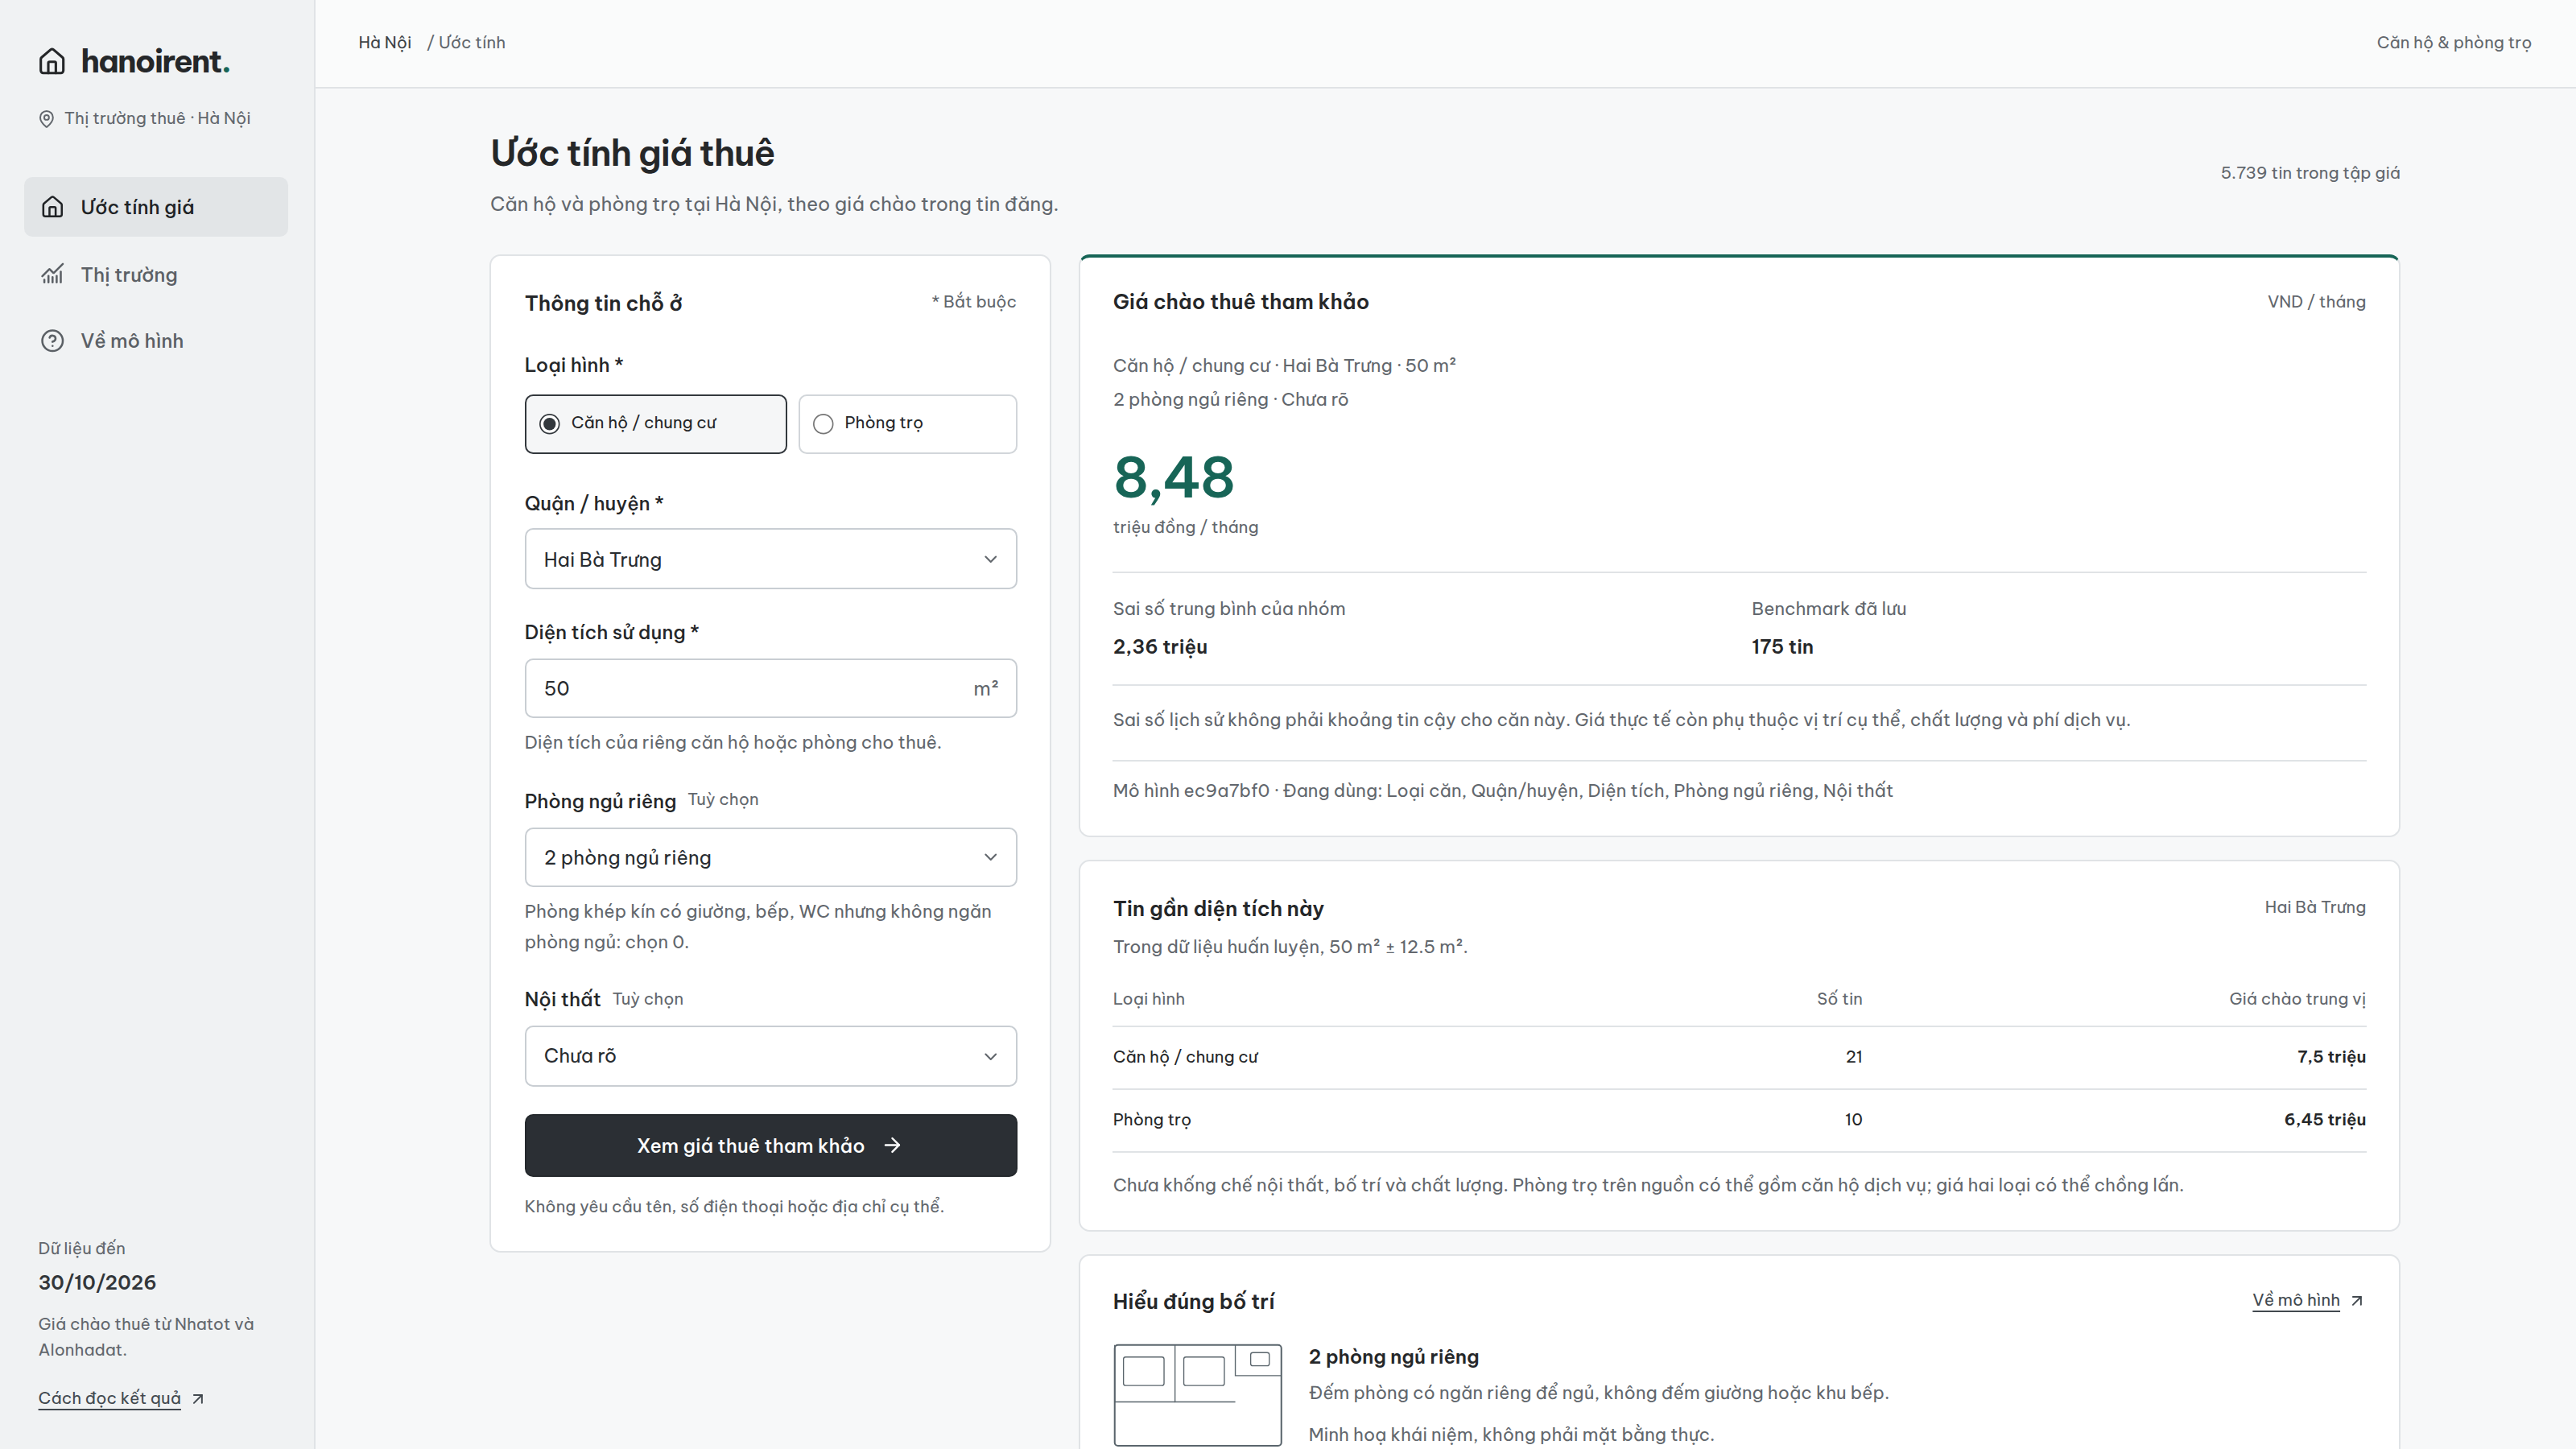
\includegraphics[width=\textwidth,height=5.6cm,keepaspectratio]{images/web-estimator.png}
\par\vspace{0.05cm}
\end{frame}
\begin{frame}{Market dashboard}
\centering
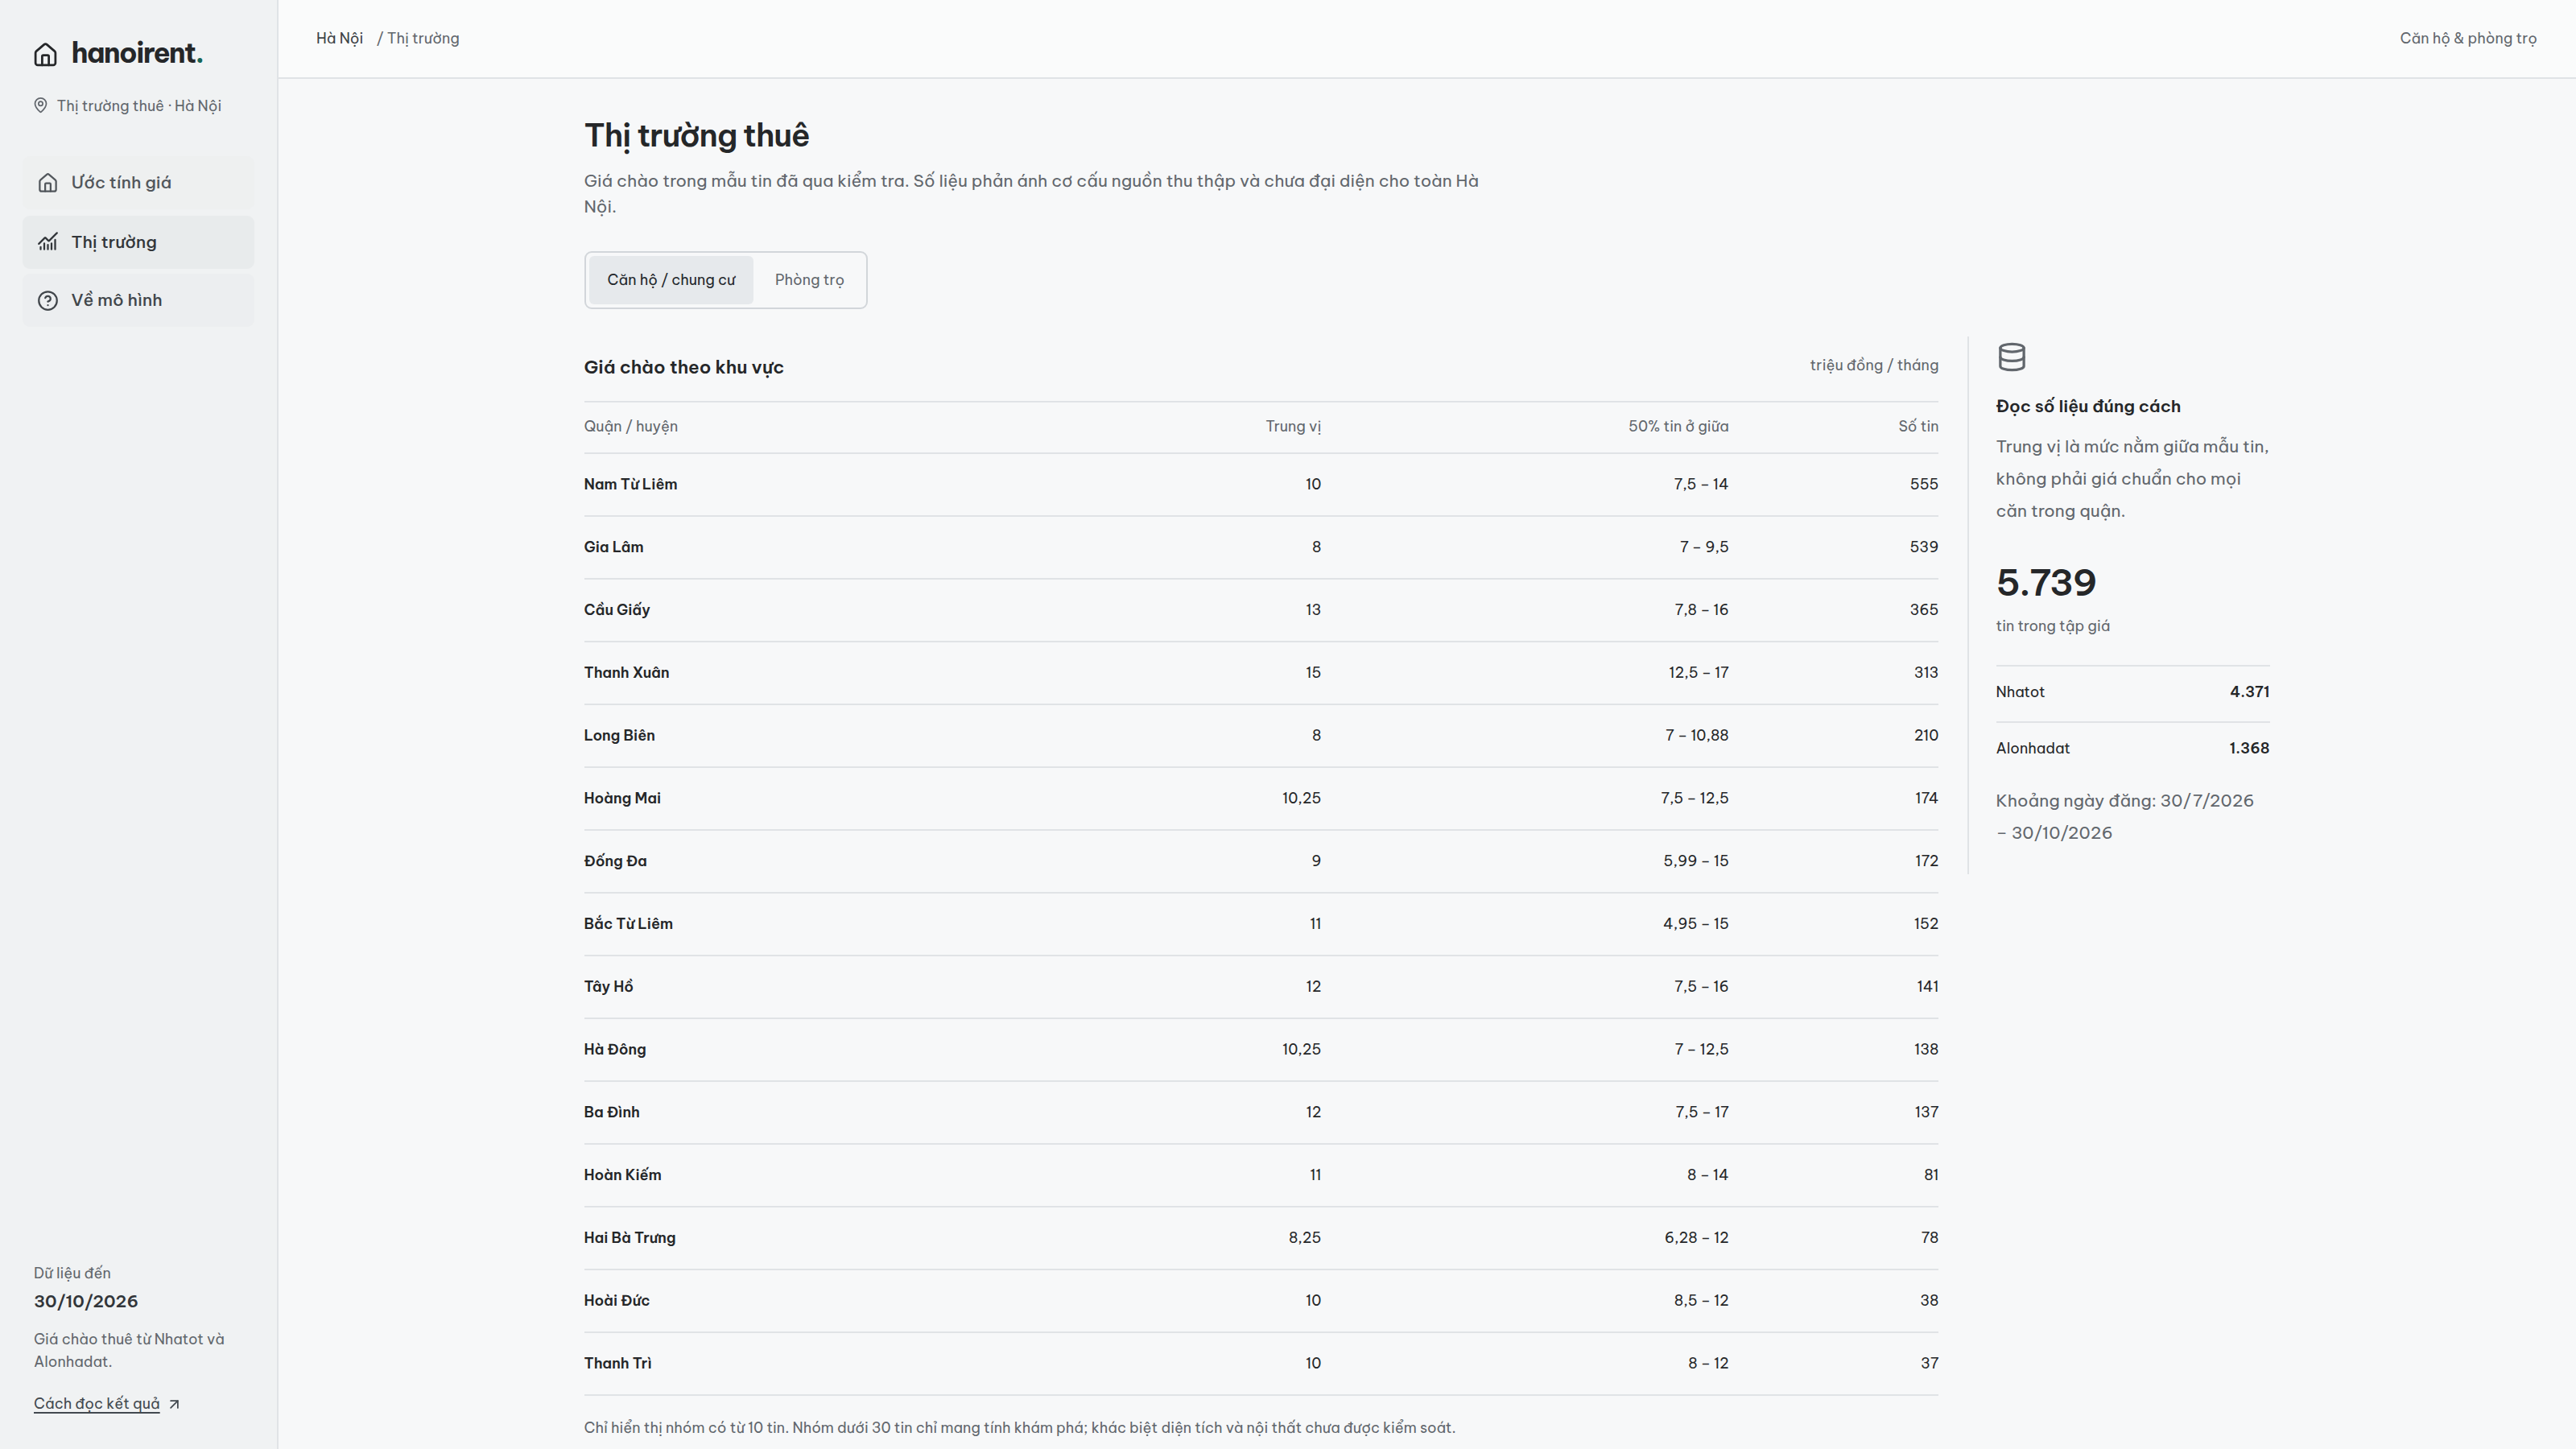
\includegraphics[width=\textwidth,height=6.0cm,keepaspectratio]{images/web-dashboard.png}
\end{frame}
\end{document}
